\documentclass{article}
\usepackage[utf8]{inputenc}
\usepackage{graphicx}
\usepackage{subcaption}
\usepackage{placeins}
\usepackage{bm}
\usepackage{amsmath}
\usepackage{tikz}
\usetikzlibrary{bayesnet}

\graphicspath{{/home/frederik/PycharmProjects/deep_restoration/plots/}}

\title{MSc. Thesis - Deep Restoration\\Paper Summary}
\date{\today}
\author{Frederik Harder}



\begin{document}

\maketitle

\section{Introduction \& Motivation}


Hierarchical feature learning has been a driving force behind recent advances in machine learning. Since the success of the model by Krizhevsky et al. \cite{alexnet}, now commonly referred to as AlexNet, at the 2012 ImageNet visual recognition challenge, deep neural networks have begun dominating computer vision and several other areas in machine learning, such as reinforcement learning and speech recognition, with more applications in active exploration. Along with this growing popularity of deep learning methods, there has been an increasing interest in visualizing these learned representations, and elucidating, what information these deep models base their decisions on. 

Especially in the field of computer vision, where learned visual representations can be easy to interpret, a number of different approaches have been published on this matter and will be discussed in some detail below. A common theme is that, in order to visualize representations at a certain layer in the network, (sometimes a subset of) the network's activations in that layer are, in some way or another, related back to the image space at the network input. This is not a trivial task, as the processing steps that transform the input up to that layer are highly non-linear and generally non-invertible. Going through a deep neural network, information from the input is compressed and details that are deemed irrelevant can be omitted. As a result, the task of reconstructing an input from the activation of a single layer is usually under-constrained and there is a class of inputs, which cause the same or nearly identical activations in the layer.

This project builds on work by Mahendran \& Vedaldi \cite{mv15, mv16}, who constrain the reconstruction problem with image priors, and aims to improve upon their results by employing more expressive priors both in image space and over the feature map activations of the network in question.

In the remainder of this section, the challenges and limitations of two major approaches to network inversion are discussed, in order to give an intuition of the task. Following that, section 2 provides an overview of the related work in this field and introduces some of the references that this project draws from. In section 3, the models introduces the used models in detail, followed by an overview of the experimental results up to this point in section 4. Section 5 specifies the future goals of the project and outlines the steps that still need to be completed, as well as pointing out some expected challenges and unresolved questions.

\subsection{Theoretical Considerations}



\subsubsection{Limitations of inverse networks}


Claim: Convolutions are not sufficient for inverting convolutions.

Argument sketch: Given a feature map as $f_{j+1}$, where $\bm{W_j}$ is toeplitz and $f_j$ is a variable with Gaussian log prior given as $\frac{1}{2} f_j^T \bm{\Sigma_{f_j}^{-1}}f_j + const$, the optimization over $f_j$ is as follows:

\begin{equation}
	\min_{f_j} \frac{1}{2} \lambda || f_{j+1} - \bm{W_j} f_j ||^2 + \frac{1}{2} f_j^T \bm{\Sigma_{f_j}^{-1}} f_j + const
\end{equation}

which resolves to 

\begin{equation}
\hat{f}_j =  \bigg( \frac{1}{\lambda}  \bm{\Sigma_{f_j}^{-1}} + \bm{W_j^T} \bm{W_j}\bigg)^{-1} \bm{W_j^T} f_{j+1}
\end{equation}

It can be shown, that $\big( \frac{1}{\lambda}  \bm{\Sigma_{f_j}^{-1}} + \bm{W_j^T} \bm{W_j}\big)^{-1} \bm{W_j^T}$ is not toeplitz (under what conditions?, why?), and therefore the optimal inverse operation is not a convolution.

Assuming no prior and going for the maximum likelihood estimate can instead be approximated with the Moore-Penrose pseudoinverse $\hat{f}_j = \bm{W_j}^+ f_{j+1}$. $\bm{W_j^{+}}$ is also not toeplitz (under what conditions?). Therefore using convolutions to approximate $\bm{W_j^{+}}$ limits reconstruction performance by design.


\subsubsection{Limitations of optimization based approaches}

\begin{itemize}
	\item non-convex optimization
	\item not clear what to optimize (MSE is not necessarily the best measure)
	\item underconstrained. priors are necessary. what priors to use is an open problem
\end{itemize}

\section{Related Work}

\begin{itemize}
	\item in detail:
		\subitem Dosovitskiy \& Brox: Inverting networks \cite{dobro_inverting, dobro_deepsim}
		\subitem Mahendran \& Vedaldi: \cite{mv15, mv16}
		\subitem Yosinsky et al.: using classifiers for generative modeling \cite{plugnplay}
	\item Gatis et al.: Style transfer using different feature map measures \cite{gatys_style}
	\item Zeiler \& Fergus: generally de-convolutional approaches should maybe be mentioned. What to they visualize, what does this approach? \cite{zeiler_fergus}
		\subitem then also Kindermans et al. (patternnet, patternrlrp) \cite{patternnet}
	\item also others (list in progress)
\end{itemize}


\section{Methods}

\subsection{Image classifiers}

Basic section on deep image classifiers coming up!

\subsubsection{AlexNet}

Overview of the AlexNet architecture coming up!

\subsubsection{Vgg16}

Overview of the Vgg16 architecture coming up!

\subsection{Modular inverting networks}

Following the work by Dosovitskiy \& Brox \cite{dobro_inverting}, a first baseline has been set using inverting networks. Here, a modular approach is used, where each module is trained to in invert a small part of the network, i.e. either a convolution operation followed by a nonlinearity, a pooling operation, or, in case of AlexNet, a local response normalization operation. These modules can then be combined and trained synchronously, where each module output computes a reconstruction loss and is fed as input to the next module, as shown in figure \ref{tikz:modinv}. Different modules have been tested and a transpose convolution, followed by a ReLU and then a convolution has performed best. Future results will follow Odena et al. \cite{odena} and use upscaling and convolution instead of a regular transpose convolution in order to prevent artifacts.

\begin{figure}
	\centering
	\resizebox{0.6\textwidth}{!}{
	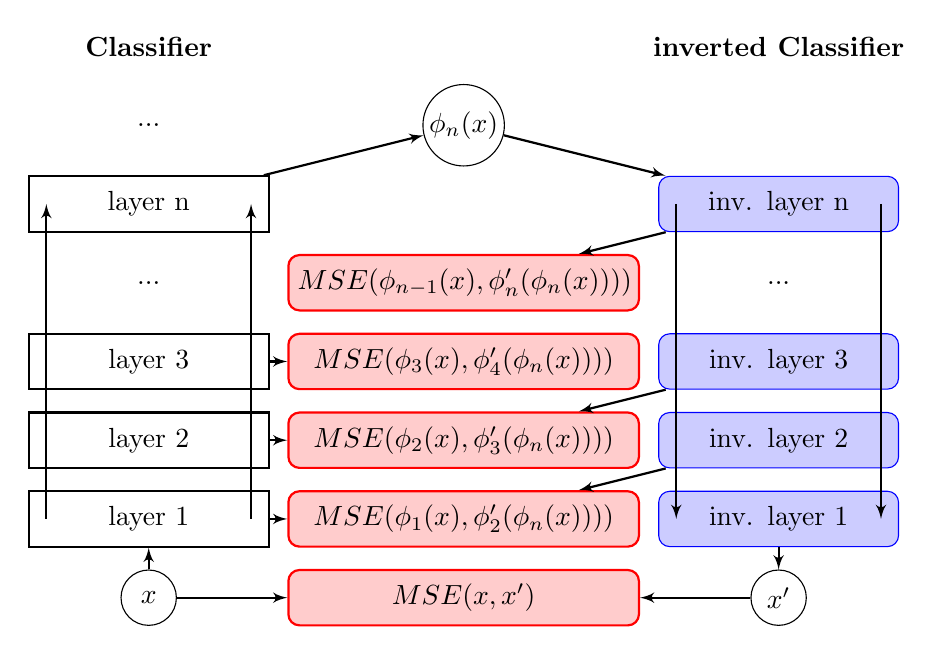
\begin{tikzpicture}
	[auto,
	net/.style ={rectangle, draw=blue, fill=blue!20, text width=3em,align=center, rounded corners, text width=8em, minimum height=2em},
	loss/.style ={rectangle, draw=red, thick, fill=red!20, text width=12em,align=center, rounded corners, minimum height=2em},
	klloss/.style ={rectangle, draw=red, thick, fill=red!20, text width=13em,align=center, rounded corners, minimum height=2em},
	dist/.style ={rectangle, draw=black, thick, text width=5em,align=center, rounded corners, minimum height=2em},
	layer/.style ={rectangle, draw=black, thick, text width=8em,align=center, minimum height=2em},
	line/.style ={draw, thick, -latex'},
	cloud/.style ={draw=red, thick, ellipse,fill=red!20,
		minimum height=1em}]
	\draw (0, -1) node[latent] (x) {$x$};
	\draw (8, -1) node[latent] (x') {$x'$};
	\draw (0, 0) node[layer] (l1) {layer 1};
	\draw (0, 1) node[layer] (l2) {layer 2};
	\draw (0, 2) node[layer] (l3) {layer 3};
	\draw (0, 3) node[] (dot) {...};
	\draw (0, 4) node[layer] (ln) {layer n};
	\draw (0, 5) node[] (dot2) {...};
	\draw (0, 6) node[] (name) {\textbf{Classifier}};
	\draw (8, 0) node[net] (l1') {inv. layer 1};
	\draw (8, 1) node[net] (l2') {inv. layer 2};
	\draw (8, 2) node[net] (l3') {inv. layer 3};
	\draw (8, 3) node[] (dot3) {...};
	\draw (8, 4) node[net] (ln') {inv. layer n};
	\draw (8, 6) node[] (name) {\textbf{inverted Classifier}};
	\draw (4, 5) node[latent] (fx) {$\phi_n (x)$};
	\draw (4, -1) node[loss] (msex) {$MSE(x, x')$};
	\draw (4, 0) node[loss] (msefx1) {$MSE(\phi_1(x), \phi_2'(\phi_n(x))))$};
	\draw (4, 1) node[loss] (msefx2) {$MSE(\phi_2(x), \phi_3'(\phi_n(x))))$};
	\draw (4, 2) node[loss] (msefx3) {$MSE(\phi_3(x), \phi_4'(\phi_n(x))))$};
	\draw (4, 3) node[loss] (msefxn) {$MSE(\phi_{n-1}(x), \phi_n'(\phi_n(x))))$};
	\draw[line] (-1.3, 0) -- (-1.3, 4);
	\draw[line] (1.3, 0) -- (1.3, 4);
	\draw[line] (6.7, 4) -- (6.7, 0);
	\draw[line] (9.3, 4) -- (9.3, 0);
	\draw[line] (ln) -- (fx);
	\draw[line] (fx) -- (ln');
	\draw[line] (x) -- (msex);
	\draw[line] (x') -- (msex);
	\draw[line] (l2') -- (msefx1);
	\draw[line] (l1) -- (msefx1);
	\draw[line] (l3') -- (msefx2);
	\draw[line] (l2) -- (msefx2);
	\draw[line] (l3) -- (msefx3);
	\draw[line] (ln') -- (msefxn);
	\draw[line] (x) -- (l1);
	\draw[line] (l1') -- (x');
	\end{tikzpicture}
	}
	\caption{Modular inverting network architecture}
	\label{tikz:modinv}
\end{figure}

\subsection{Optimization based methods}

The central approach to network visualization is based on work by Mahendran \& Vedaldi \cite{mv15, mv16}. Their method, illustrated in figure \ref{tikz:mv}, optimizes a \textit{pre-image} variable to match one of its feature map representations with that of an image, while constraining the \textit{pre-image} additionally by a hand-crafted natural image prior. These results have been reproduced, with the goal of improving upon them by using learned priors instead of handcrafted ones. In addition to a natural image prior, priors trained on the feature maps will be used to constrain the problem further and hopefully lead to better reconstructions as a result. This setup is shown in figure \ref{tikz:mv+}.
	
\begin{figure}
	\centering
	\resizebox{0.6\textwidth}{!}{
	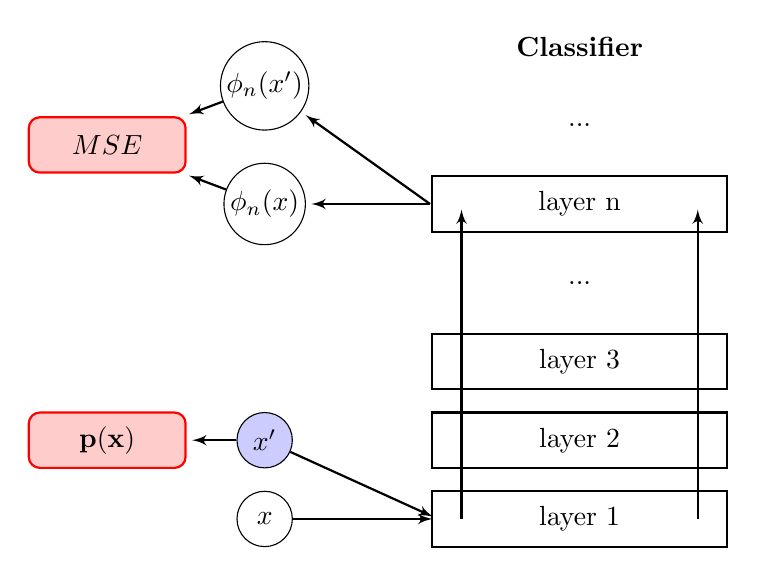
\begin{tikzpicture}
	[auto,
	net/.style ={rectangle, draw=blue, thick, fill=blue!20, text width=3em,align=center, rounded corners, minimum height=2em},
	loss/.style ={rectangle, draw=red, thick, fill=red!20, text width=5em,align=center, rounded corners, minimum height=2em},
	klloss/.style ={rectangle, draw=red, thick, fill=red!20, text width=13em,align=center, rounded corners, minimum height=2em},
	dist/.style ={rectangle, draw=black, thick, text width=5em,align=center, rounded corners, minimum height=2em},
	layer/.style ={rectangle, draw=black, thick, text width=10em,align=center, minimum height=2em},
	line/.style ={draw, thick, -latex',shorten >=2pt},
	cloud/.style ={draw=red, thick, ellipse,fill=red!20,
		minimum height=1em}]
	\draw (-1.8, 0) node[latent] (x) {$x$};
	\draw (-1.8, 1) node[latent, fill=blue!20] (x') {$x'$};
	\draw (2.2, 0) node[layer] (l1) {layer 1};
	\draw (2.2, 1) node[layer] (l2) {layer 2};
	\draw (2.2, 2) node[layer] (l3) {layer 3};
	\draw (2.2, 3) node[] (dot) {...};
	\draw (2.2, 4) node[layer] (ln) {layer n};
	\draw (2.2, 5) node[] (dot2) {...};
	\draw (2.2, 6) node[] (name) {\textbf{Classifier}};
	\draw (-1.8, 4) node[latent] (fx) {$\phi_n (x)$};
	\draw (-1.8, 5.5) node[latent] (fx') {$\phi_n (x')$};
	\draw (-3.8, 1) node[loss] (px) {$\mathbf{p(x)}$};
	\draw (-3.8, 4.75) node[loss] (mse) {$MSE$};
	\draw[line] (x) -- (0.4, 0);
	\draw[line] (x') -- (0.4, 0);
	\draw[line] (0.3, 4) -- (fx);
	\draw[line] (0.3, 4) -- (fx');
	\draw[line] (fx) -- (mse);
	\draw[line] (fx') -- (mse);
	\draw[line] (x') -- (px);
	\draw[line] (0.7, 0) -- (0.7, 4);
	\draw[line] (3.7, 0) -- (3.7, 4);
	\end{tikzpicture}
	}
	\caption{Model by Mahendran \& Vedaldi \cite{mv15, mv16}}
	\label{tikz:mv}
\end{figure}

\begin{figure}
	\centering
	\resizebox{0.8\textwidth}{!}{
	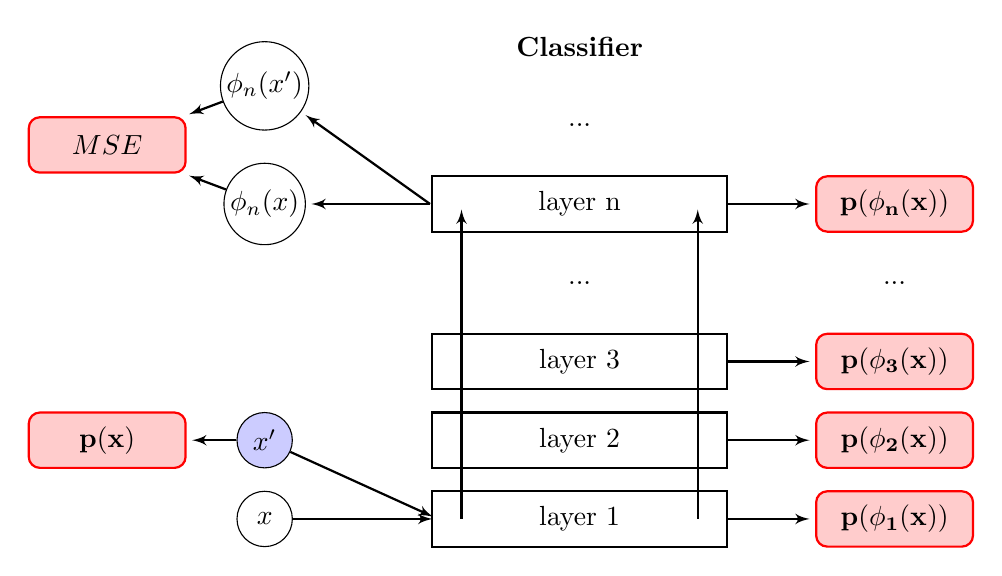
\begin{tikzpicture}
	[auto,
	net/.style ={rectangle, draw=blue, thick, fill=blue!20, text width=3em,align=center, rounded corners, minimum height=2em},
	loss/.style ={rectangle, draw=red, thick, fill=red!20, text width=5em,align=center, rounded corners, minimum height=2em},
	klloss/.style ={rectangle, draw=red, thick, fill=red!20, text width=13em,align=center, rounded corners, minimum height=2em},
	dist/.style ={rectangle, draw=black, thick, text width=5em,align=center, rounded corners, minimum height=2em},
	layer/.style ={rectangle, draw=black, thick, text width=10em,align=center, minimum height=2em},
	line/.style ={draw, thick, -latex',shorten >=2pt},
	cloud/.style ={draw=red, thick, ellipse,fill=red!20,
		minimum height=1em}]
	\draw (-4, 0) node[latent] (x) {$x$};
	\draw (-4, 1) node[latent, fill=blue!20] (x') {$x'$};
	\draw (0, 0) node[layer] (l1) {layer 1};
	\draw (0, 1) node[layer] (l2) {layer 2};
	\draw (0, 2) node[layer] (l3) {layer 3};
	\draw (0, 3) node[] (dot) {...};
	\draw (0, 4) node[layer] (ln) {layer n};
	\draw (0, 5) node[] (dot2) {...};
	\draw (0, 6) node[] (name) {\textbf{Classifier}};
	\draw (-4, 4) node[latent] (fx) {$\phi_n (x)$};
	\draw (-4, 5.5) node[latent] (fx') {$\phi_n (x')$};
	\draw (-6, 1) node[loss] (px) {$\mathbf{p(x)}$};
	\draw (-6, 4.75) node[loss] (mse) {$MSE$};
	\draw (4, 0) node[loss] (pfx1) {$\mathbf{p(\phi_1(x))}$};
	\draw (4, 1) node[loss] (pfx2) {$\mathbf{p(\phi_2(x))}$};
	\draw (4, 2) node[loss] (pfx3) {$\mathbf{p(\phi_3(x))}$};
	\draw (4, 3) node[] (dot3) {...};
	\draw (4, 4) node[loss] (pfxn) {$\mathbf{p(\phi_n(x))}$};
	\draw[line] (x) -- (-1.8, 0);
	\draw[line] (x') -- (-1.8, 0);
	\draw[line] (-1.9, 4) -- (fx);
	\draw[line] (-1.9, 4) -- (fx');
	\draw[line] (fx) -- (mse);
	\draw[line] (fx') -- (mse);
	\draw[line] (x') -- (px);
	\draw[line] (-1.5, 0) -- (-1.5, 4);
	\draw[line] (1.5, 0) -- (1.5, 4);
	\draw[line] (l1) -- (pfx1);
	\draw[line] (l2) -- (pfx2);
	\draw[line] (l3) -- (pfx3);
	\draw[line] (ln) -- (pfxn);
	\end{tikzpicture}
	}
	\caption{Extension of Mahendran \& Vedaldi with feature map priors}
	\label{tikz:mv+}
\end{figure}
	
\subsection{Priors}


\subsubsection{Mahendran \& Vedaldi's work and handcrafted image priors}

In \cite{mv15}, the authors employ an optimization method, using a normalized mean squared error loss on the feature maps and two image priors. 

The normalized mean squared error takes the form

\begin{equation}
	|| \Phi(\sigma \mathbf{x}) - \Phi_0 ||_2^2 / ||\Phi_0||^2_2
\end{equation}

where $\Phi_0$ is the feature map representation of the target image and $\Phi(\sigma \mathbf{x})$ is the representation of the re-scaled \textit{pre-image} $\mathbf{x}$. The scaling factor $\sigma = 2.7098\mathrm{e+}4$ is chosen as the average Euclidean norm of natural images in the training set to the effect that $\mathbf{x}$ has roughly unitary Euclidean norm. Dividing the mean squared error by the squared Euclidean norm of the target image confines errors near an optimum to the interval $[0,1]$. This predictability can be convenient when considering the scaling of the priors and as a result, the same normed mean squared error loss has been adopted for the experiments using learned priors, discussed below.

The authors constrain the optimization of the feature level error with two hand-designed priors. The first one is an $\alpha$-norm prior, defined as 

\begin{equation}
\mathcal{R}_\alpha(\mathbf{x}) = ||\mathbf{x} - \mathrm{mean}(\mathbf{x}) ||^\alpha_\alpha
\end{equation}
 
It is meant to limit the overall range of pixel values. Results are reported with $\alpha=6$.

In addition, a total variation prior is used, which penalizes the difference between neighboring pixels and thus encourages smoothness in the pre-image. It takes the following form, with $\beta = 2$ being chosen in most experiments:

\begin{equation}
\mathcal{R}_{V^\beta}(\mathbf{x}) = \sum_{i,j} \big( (x_{i,j+1} - x_{i,j})^2 + (x_{i+1,j} - x_{i,j})^2 \big)^{\frac{\beta}{2}}
\end{equation}


In their follow-up publication \cite{mv16}, the authors maintain the MSE loss and total variation prior, but refine the range prior to

\begin{equation}
	N_\alpha(\mathbf{x}) = \sum_{i,j}\bigg( \sum_{k} \mathbf{x}_{ijk}^2 \bigg)^{\frac{\alpha}{2}}
\end{equation}

where $i,j$ are pixel positions and $k$ denotes the channel. The authors argue that this version resolves a problem of color bias introduced by the alpha norm prior, because unlike the previous one, it is isotropic in RGB space. They couple this soft constraint with a hard one, which enforces $\sqrt{\sum_k \mathbf{x}_{ijk}^2} \leq B_{+}$ for each image position $(i,j)$. They also develop the weighting of the different parameters further and introduce an additional regularization method called jittering, which makes small shifts to the pre-image on each iteration and produces crisper images overall. Jittering may be considered in combination with learned priors at a future point and a detailed treatment of the method will be provided, but is omitted for now.

\subsubsection{ICA based sparse coding priors}

In his paper on the method of score matching \cite{hyvarinen2003}, the author introduces a model for image patches $\mathbf{x}_{(k)}$ based on over-complete independent component analysis (ICA). The log probability of is defined, using the function $G(s) = - \log \cosh(s)$ and an unspecified normalizing constant $Z$. 

\begin{equation}
	p(\mathbf{x}_{(k)}) = \exp (Z(\mathbf{w_1},...,\mathbf{w_N}, \alpha_1, ... , \alpha_N)) \prod_{i=1}^{N} \exp \big(G(\mathbf{w}_i^T \mathbf{x}_{(k)}) \big)^{\alpha_i}  
	\label{eq:ica_patch}
\end{equation}

Following the derivations of \cite{hyvarinen2003}, this prior for image patches can be trained via score matching, using mini-batch gradient descent, by minimizing the sampled loss function $\tilde{J}$ over a training set of image patches. For this purpose the first two derivatives of $G$ are computed as $g(s) = - \tanh(s)$ and $g'(s) = - \cosh(s)^{-2}$.

\begin{equation}
\begin{aligned}
\tilde{J} = \sum_{k=1}^{m} \alpha_k \frac{1}{T} \sum_{t=1}^{T} g'(\mathbf{w}_k^T \mathbf{x}_{(t)}) + \frac{1}{2} \sum_{j,k = 1}^{m} \alpha_j \alpha_k \mathbf{w}_j^T \mathbf{w}_k \frac{1}{T} \sum_{t=1}^{T} g(\mathbf{w}_k^T \mathbf{x}_{(t)}) g(\mathbf{w}_j^T \mathbf{x}_{(t)})
\end{aligned}
\label{eq:jtilde}
\end{equation}

The trained patch prior can then be turned into an image prior, by the same consideration, that is used in \cite{foe}. Viewing the image as a Markov random field with a node for each pixel position and a patch centered at each position, nodes are connected, iff they share a patch. As the patch prior in equation (\ref{eq:ica_patch}) is strictly positive and the patches constitute the maximal cliques of the Markov random field, the patch prior can serve as a clique potential and the probability of the field is proportional to the product of its clique potentials (source).

\begin{equation}
\begin{aligned}
p(\mathbf{x}) \propto& \prod_{k=1}^K \exp (Z(\mathbf{w_1},...,\mathbf{w_N}, \alpha_1, ... , \alpha_N)) \prod_{i=1}^{N} \exp \big(G(\mathbf{w}_i^T \mathbf{x}_{(k)}) \big)^{\alpha_i}  \\
\propto& \prod_{k=1}^K \prod_{i=1}^{N} \exp \big(G(\mathbf{w}_i^T \mathbf{x}_{(k)}) \big)^{\alpha_i}  \\
\log p(\mathbf{x}) \propto& \sum_{k=1}^K \sum_{i=1}^{N} \alpha_i G(\mathbf{w}_i^T \mathbf{x}_{(k)}) \\
\end{aligned}
\label{eq:ica_img}
\end{equation}



\subsubsection{Fields of experts priors}

The field of experts prior developed by Roth and Black \cite{foe} is a patch based prior of the form 

\begin{equation}
	p(\mathbf{x}) = \frac{1}{Z(\bm{\Theta})} \prod_{k}^K \prod_{i=1}^{N} \phi_i (\mathbf{w}_i^T \mathbf{x}_{(k)} ; \alpha_i) \\
\end{equation}

for a set of $K$ equally sized patches $\mathbf{x}_{(k)}$, where $\phi_i$ are Student's t distributions $\phi_i(\mathbf{w}_i^T \mathbf{x}_{(k)} ; \alpha_i) = (1 + \frac{1}{2}(\mathbf{w}_i^T \mathbf{x}_{(k)})^2 )^{-\alpha_i}$, parameterized by $\mathbf{w}$ and $\mathbf{\alpha}$ and $Z(\bm{\Theta})$ is a normalizing factor\footnote{In \cite{foe}, $\mathbf{J}$ is used in place of $\mathbf{w}$, but the notation is changed here, to match \cite{hyvarinen2003}}. 

Looking at the prior for an individual patch $\mathbf{x}_{(k)}$, the log likelihood can be derived up to an additive constant. This makes it possible to define the prior identically to the over-complete independent component analysis discussed above, excepting the different definition for function $G$. 

\begin{equation}
\begin{aligned}
	p(\mathbf{x}_{(k)}) =& \frac{1}{Z(\bm{\Theta})} \prod_{i=1}^{N} \phi_i (\mathbf{w}_i^T \mathbf{x}_{(k)} ; \alpha_i) \\
	=& \frac{1}{Z(\bm{\Theta})} \prod_{i=1}^{N} \bigg( 1 + \frac{1}{2}(\mathbf{w}_i^T \mathbf{x}_{(k)})^2 \bigg)^{-\alpha_i} \\
	\log p(\mathbf{x}_{(k)}) =& \sum_{i=1}^{N} -\alpha_i \log \bigg( 1 + \frac{1}{2}(\mathbf{w}_i^T \mathbf{x}_{(k)})^2 \bigg)  - \log Z(\bm{\Theta}) \\
	\propto& \sum_{i=1}^{N} -\alpha_i \log \bigg( 1 + \frac{1}{2}(\mathbf{w}_i^T \mathbf{x}_{(k)})^2 \bigg) \\
		\propto& \sum_{i=1}^{N} \alpha_i G(\mathbf{w}_i^T \mathbf{x}_{(k)})
\end{aligned}
\end{equation}

Computing the derivatives of $G$ then allows for the training of parameters $\mathbf{w}$ and $\alpha$ via score matching.


\begin{equation}
\begin{aligned}
	G(s) =& - \log(1 + \frac{1}{2} s^2) \\
	g(s) =& - \frac{2s}{s^2 + 2} \\
	g'(s) =& \frac{2(s^2 - 2)}{(s^2 + 2)^2}
\end{aligned}
\end{equation}

Directly following Hyvarinen 2003, equations (11) and (12), this results in the same sampled loss function $\tilde{J}$, shown in equation (\ref{eq:jtilde}), which finds the optimal $\mathbf{w}$ and $\alpha$ for a set of natural image patches, when minimized.


\section{Results (clear split from methods \& discussion in progress)}

\subsection{Feature map statistics}


\begin{figure}
	\centering
	\begin{subfigure}[b]{0.3\textwidth}
		\includegraphics[width=\textwidth]{covariance/avg_cov_pool5_small.png}
		\caption{Average covariance \\~}
		\label{fig:cov}
	\end{subfigure}
	~
	\begin{subfigure}[b]{0.3\textwidth}
		\includegraphics[width=\textwidth]{covariance/inv_avg_cov_pool5_lin_small.png}
		\caption{Inverse average covariance}
		\label{fig:inv_cov}
	\end{subfigure}
	\caption{both figures are based on flattened feature maps in the fifth 7 by 7 pooling layer of VGG16 over 200 images}
	\label{fig:cov_plots}
\end{figure}

In an initial investigation, three feature map characteristics were looked at. The average covariance and its inverse, shown in figure \ref{fig:cov_plots}, substantiate an assumption of spatial stationarity (ground in math) in the feature map activation. Border effects are visible, especially in the inverse matrix, but leaving these aside, the inverse is close to toeplitz, which is expected to become more accurate for larger sets of images. (and this matters because math). This finding serves to motivate convolutional and patch-based priors. Gram matrices and sparsity statistics of the feature maps were also evaluated, and may be used at a later stage in evaluating the trained feature map priors.

\subsection{Modular inverting networks}

\begin{figure}
	\centering
	\includegraphics[width=0.8\textwidth]{"temp/vgg depth progression"}
	\caption{on the left: original image, then: inverse networks reconstructions based on VGG16 feature maps from pooling layers 1, 2, and 3 (will need more detail \& deeper layers)}
	\label{fig:invert_net_progression}
\end{figure}

The inverting networks were trained on 48000 images of the 2012 ImageNet validation set, with the remaining 2000 set aside for testing. All training runs used the Adam optimizer \cite{adam} with a learning rate of $3\mathrm{e-}4$. Models were trained both on the AlexNet and the VGG16 classifier.  Figure \ref{fig:invert_net_progression} shows reconstructions from the first three pooling layers of VGG16, illustrating, how image details fail to be recovered from deeper layers.

Besides setting a baseline in terms of reconstruction quality, this approach is also intended to explore two questions. The first minor insight concerns the performance of stacked modules that were trained individually based on feature map pairs as compared to models, which are trained together. As figure \ref{fig:stack_v_sync} shows, simultaneous training yields better results. 
% (possibly trivial and to be dropped)

The second and major incentive is to motivate the use of constraints in the intermediate feature map layers. For this purpose, the modules have been trained end to end, leaving out all intermediate losses. A comparison with stacked modules is shown in figure \ref{fig:stack_v_end2end}. This result shows, that constraining the intermediate representations in the model to match the feature maps of the classifier to be inverted can lead to overall better reconstructions. It is therefore reasonable to assume that the same will hold in the following approach using optimization based methods.

Because differences between image and reconstruction can be quite small, two difference measures have been added. The first is a color/channel accurate measure, showing the difference between image and reconstruction, renormalized to the interval [0,1]. So if, for example, the reconstructed image has less blue in it, the measure will be blue. Areas without error (or equal errors across channels) are gray. The second difference measure is the renormalized absolute difference, which highlights areas with errors more clearly. Areas without error are black. Given renormalization,  pixel intensity only informs about relative error within the image, not absolute error compared to other images. Without normalization, the errors were hardly visible. The figures are ordered left to right as: image, reconstruction, color measure, absolute measure. 



\begin{figure}
	\centering
	\includegraphics[width=0.8\textwidth]{"temp/stacked_v_synched_alexnet"}
	\caption{top row: modules trained in parallel, bottom row: stacked modules.
		left to right: original image, reconstruction from AlexNet, two pixel error measures for visualization}
	\label{fig:stack_v_sync}
\end{figure}

\begin{figure}
	\centering
	\includegraphics[width=0.8\textwidth]{"temp/stacked_v_end2end_vgg"}
	\caption{Top row: end to end trained model, bottom row: stacked modules. 
		left to right: original image, reconstruction from the first VGG pooling layer, two pixel error measures for visualization}
	\label{fig:stack_v_end2end}
\end{figure}



\subsection{Optimization based reconstruction}

An ICA-based image prior with 512 filters, shown in figure \ref{fig:first_ica_filters}, has been used for performing initial reconstructions from the first and fourth layer of AlexNet. The results are displayed in figures \ref{fig:ica_mv_l1} and \ref{fig:ica_mv_l4}. Both are trained using the Adam optimizer. The first layer reconstruction used a stable learning rate of $0.004$ over $5000$ iterations, while for the fourth layer, a decreasing learning rate was used over $10000$ iterations ($0.01$ at the beginning, $4\mathrm{e-}3$ at iteration $1000$, $1\mathrm{e-}3$ at $1200$, $4\mathrm{e-}4$ at $3000$, $1\mathrm{e-}4$ at $6000$ and $4\mathrm{e-}5$ at $9000$). The same normed mean squared error loss as in \cite{mv15} is used and relative to it, the ICA prior is weighted at $1\mathrm{e-}4$ in the first layer and at $1\mathrm{e-}3$ in the fourth. A comparison to the results of \cite{mv16}, as well as an exhaustive treatment of all network layers, is in progress.

\begin{figure}
	\centering
	\includegraphics[width=0.9\textwidth]{"temp/overcomplete_ica_filters"}
	\caption{Subset of the 512 filters from an over-complete ICA prior}
	\label{fig:first_ica_filters}
\end{figure}


\begin{figure}
	\centering
	\begin{subfigure}[b]{\textwidth}
		\centering
		\includegraphics[width=0.9\textwidth]{"temp/ica-mv15-alex-conv1"}
		\caption{224x224 pixel image}
	\end{subfigure}
	
	\begin{subfigure}[b]{\textwidth}
		\centering
		\includegraphics[width=0.9\textwidth]{"temp/ica-mv15-alex-conv1-detail"}
		\caption{56x56 pixel detailed view}
	\end{subfigure}
	\caption{Comparison of reconstructions from the first layer (Convolution + ReLU) of AlexNet. Left to right: original image, ICA image prior, reproduction of \cite{mv15}}
	\label{fig:ica_mv_l1}
\end{figure}

\begin{figure}
	\centering
	\includegraphics[width=0.9\textwidth]{"temp/ica-mv15-alex-conv4"}
	\caption{Comparison of reconstructions from the fourth convolutional layer of AlexNet in detail. Left to right: original image, ICA image prior, reproduction of \cite{mv15}}
	\label{fig:ica_mv_l4}
\end{figure}



\FloatBarrier
\section{Next steps and research goals}

\subsection{Immediate next steps:}

The training of image and feature map priors based on over-complete ICA is set up and will be completed shortly. There is one potentially unresolved problem with regards to the patch sizes on feature maps. Given that the number of channels grows quickly, the patches should be chosen as small as possible. The receptive field size in the previous layer seems like a good first guess. Should the number of patch features grow too large regardless, separate priors for subsets of channels may have to be considered. This, however, would make independence assumptions that are almost certainly wrong and can hopefully be avoided. 

When the priors are trained, a prime concern will be the adequate relative weighting in optimization based reconstruction, as each one of them represents an un-normalized negative log probability and as a result can vary greatly in scale. If a principled approach is not found, parameter exploration schemes will have to be designed.

Experiments will then investigate the quality of reconstructions following \cite{mv16} with learned priors perhaps augmenting, but most likely replacing the handcrafted ones.
If these efforts prove fruitful, related applications like activation maximization and caricaturization \cite{mv16} can be explored in a quick follow-up. If, instead, the results point to limitations of the prior model, alternative models will need to be explored immediately. Here I propose two options: The field of experts model is closely related to the model using ICA based filters, but uses Student-t experts instead of a logistically distributed components and is well established as a model. The second option comes from \cite{plugnplay}, which uses denoising auto-encoders to approximate the gradient of natural image priors. This should also work on feature maps and is distinct, in that it is not explicitly a patch-based approach. On the other hand, training times may become more of a concern in that case.

\subsection{Goals:}

The minimal empirical project goal at this point is the reproduction of the experiments conducted by \cite{mv16}, with the use of learned image and feature map priors.

A variety of new experiments could be enabled with a good sampling technique. As far as I am aware, unfortunately, neither the patch-based methods, nor the DAE prior lend themselves very well to this task. The highest goal, of sampling images jointly from weighted priors at different feature maps poses an additional problem, which I can currently offer no good solution to. Of course the modes of these distributions can be explored through optimizing pre-images. 
Generative models, for instance Variational Auto-Encoders, can be trained on individual feature maps and serve as targets for optimization based approaches or as inputs to inverting networks. This could show, how the distribution of feature map activations corresponds to natural images.

The fact that the related literature up to this point has mostly been concerned with classical convolutional networks such as AlexNet or Vgg16, while the state of the art has moved on. It may therefore be fruitful to apply the methods developed here to inception-based or ResNet models for comparison.

A wider review of related work may also provide some additional setups that can be improved with priors. (A day or two of reading may be necessary though) 

\subsection{Some thoughts on evaluating priors}

\begin{itemize}
	\item measures:
	\subitem reconstruction MSE in image space compared with M\&V is a bit of a cheap shot, because that's not really something they set out to improve (they do report something which they call reconstruction error, but which, from the numbers and everything has to be the representation MSE). also, these scores will be abysmal regarding deeper layers, no matter which approach is taken.
	\subitem for Dosovitskiy, MSE is fair game, but might be harder, because the explicitly optimize for it. So qualitatively nicer reconstructions might still lose that contest.
	\subitem Structural similarity index might be an option, because it's at least translation invariant (right?). It is also perception focused, which might not be all bad, but is not necessarily all that interesting. As it is an accumulated measure, maybe some of its components are useful. (details follow)
	\item expectations:
	\subitem the results by M\&V on lower layer reconstructions look really good. not sure if learned priors can actually beat that. maybe in conjunction with some of the M\&V parts.
	\subitem on lower layers, feature map priors could become increasingly important and these should likely show the first improvements
	\item very rough test setups:
	\subitem test each prior on natural image feature maps to get an idea of the spread of values
	\subitem all priors can be tested individually, e.g. with the M\&V image priors in place. maybe some layers have more of an impact than others? (deep vs. shallow)
	\subitem To get to the point where all priors are used in the model, maybe it's a good idea to add them iteratively. The question then is, do you start deep or shallow? maybe just start with whatever worked best previously. 
	\subitem 
\end{itemize}

\begin{thebibliography}{9}



\bibitem{dobro_deepsim} Dosovitskiy, A., \& Brox, T. (2016). Generating images with perceptual similarity metrics based on deep networks. In Advances in Neural Information Processing Systems (pp. 658-666).

\bibitem{dobro_inverting} Dosovitskiy, A., \& Brox, T. (2016). Inverting visual representations with convolutional networks. In Proceedings of the IEEE Conference on Computer Vision and Pattern Recognition (pp. 4829-4837).

\bibitem{gatys_style} Gatys, L. A., Ecker, A. S., \& Bethge, M. (2015). A neural algorithm of artistic style. arXiv preprint arXiv:1508.06576.

\bibitem{hyvarinen2003} Hyvärinen, A. (2005). Estimation of non-normalized statistical models by score matching. Journal of Machine Learning Research, 6(Apr), 695-709.

\bibitem{adam} Kingma, D., \& Ba, J. (2014). Adam: A method for stochastic optimization. arXiv preprint arXiv:1412.6980.

\bibitem{alexnet} Krizhevsky, A., Sutskever, I., \& Hinton, G. E. (2012). Imagenet classification with deep convolutional neural networks. In Advances in neural information processing systems (pp. 1097-1105).

\bibitem{mv15} Mahendran, A., \& Vedaldi, A. (2015). Understanding deep image representations by inverting them. In Proceedings of the IEEE conference on computer vision and pattern recognition (pp. 5188-5196).

\bibitem{mv16} Mahendran, A., \& Vedaldi, A. (2016). Visualizing deep convolutional neural networks using natural pre-images. International Journal of Computer Vision, 120(3), 233-255.

\bibitem{plugnplay} Nguyen, A., Yosinski, J., Bengio, Y., Dosovitskiy, A., \& Clune, J. (2016). Plug \& play generative networks: Conditional iterative generation of images in latent space. arXiv preprint arXiv:1612.00005.

\bibitem{odena} Odena, A. Dumoulin, V. \& Olah, C. (2016) Deconvolution and Checkerboard Artifacts. Distill. http://doi.org/10.23915/distil

\bibitem{foe} Roth, S., \& Black, M. J. (2005, June). Fields of experts: A framework for learning image priors. In Computer Vision and Pattern Recognition, 2005. CVPR 2005. IEEE Computer Society Conference on (Vol. 2, pp. 860-867). IEEE.

\bibitem{vgg16} Simonyan, K., \& Zisserman, A. (2014). Very deep convolutional networks for large-scale image recognition. arXiv preprint arXiv:1409.1556.

\bibitem{zeiler_fergus} Zeiler, M. D., \& Fergus, R. (2014, September). Visualizing and understanding convolutional networks. In European conference on computer vision (pp. 818-833). Springer, Cham.

\bibitem{patternnet} Kindermans, P. J., Schütt, K. T., Alber, M., Müller, K. R., \& Dähne, S. (2017). PatternNet and PatternLRP--Improving the interpretability of neural networks. arXiv preprint arXiv:1705.05598.

\end{thebibliography}








\end{document}